
% header %{{{1

\documentclass[tikz, border=1mm]{standalone}

\usepackage{amsmath}

\usepackage{tikz}

\usetikzlibrary{calc,angles,quotes,intersections,shapes.geometric}

\usepackage{tkz-euclide}

% document %{{{1

% opening %{{{2

\begin{document}
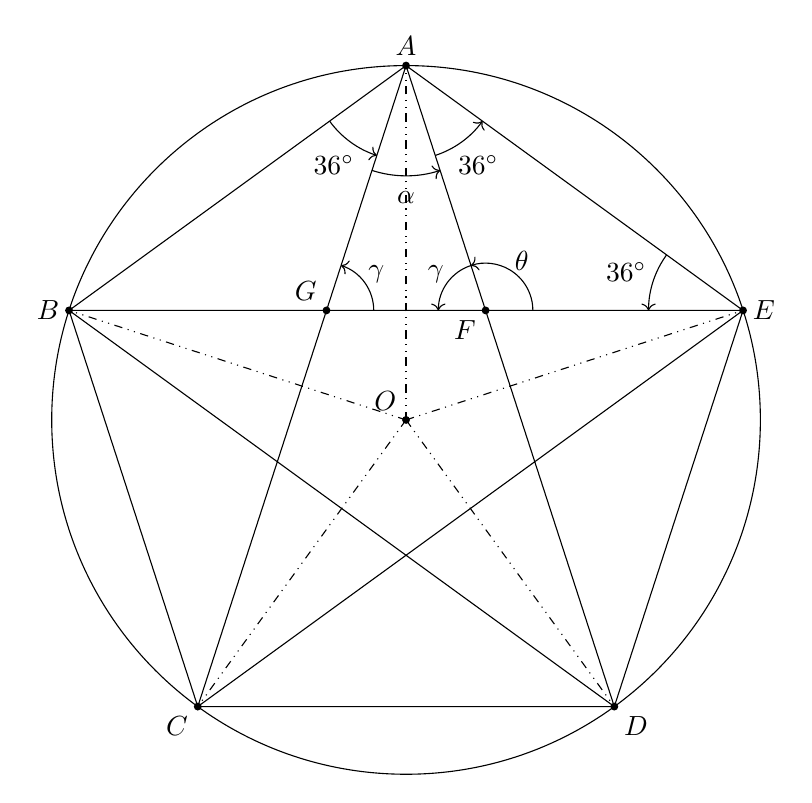
\begin{tikzpicture}[scale=1.0]

% parameters %{{{2

	\def\numsides{5}
	\def\radius{4.5}
	\def\rotation{90}

% coordinates %{{{2

	\coordinate (O) at (0,0);

	\foreach \i in {1,...,\numsides} {
		\coordinate (P\i) at ({360/\numsides*(\i-1)+\rotation}:\radius);
	}

% intersections %{{{2

	\tkzInterLL(P2,P5)(P1,P4)\tkzGetPoint{F}
	\tkzInterLL(P2,P5)(P1,P3)\tkzGetPoint{G}

% circle %{{{2

	\draw (O) circle (\radius);

% polygon %{{{2

	\draw (P1) \foreach \i in {2,...,\numsides} { -- (P\i) } -- cycle;

% radiuses %{{{2

	\foreach \i in {1,...,\numsides} { \draw[dashdotdotted] (O) -- (P\i); }

% pentagram %{{{2

	\draw[solid] (P1) -- (P3) -- (P5) -- (P2) -- (P4) -- cycle;

% points, dots, vertices %{{{2

	\fill (O) circle (0.5mm);
	\fill (F) circle (0.5mm);
	\fill (G) circle (0.5mm);
	\foreach \i in {1,...,\numsides} { \fill (P\i) circle (0.5mm); }

% points, dots, vertices labels %{{{2

	\node[above left] at (O) {$O$};
	\node[below left] at (F) {$F$};
	\node[above left] at (G) {$G$};

	\node[above] at (P1) {$A$};
	\node[left] at (P2) {$B$};
	\node[below left] at (P3) {$C$};
	\node[below right] at (P4) {$D$};
	\node[right] at (P5) {$E$};

% angles labels %{{{2

	\pic[draw, ->, "$36^\circ$", angle radius=1.2cm, angle eccentricity=1.3]
	{angle = P4--P1--P5};

	\pic[draw, ->, "$36^\circ$", angle radius=1.2cm, angle eccentricity=1.3]
	{angle = P1--P5--P2};

	\pic[draw, ->, "$36^\circ$", angle radius=1.2cm, angle eccentricity=1.3]
	{angle = P2--P1--P3};

	\pic[draw, ->, "$\alpha$", angle radius=1.4cm, angle eccentricity=1.2]
	{angle = P3--P1--P4};

	\pic[draw, ->, "$\gamma$", angle radius=0.6cm, angle eccentricity=1.3]
	{angle = P5--G--P1};

	\pic[draw, ->, "$\gamma$", angle radius=0.6cm, angle eccentricity=1.3]
	{angle = P1--F--P2};

	\pic[draw, ->, "$\theta$", angle radius=0.6cm, angle eccentricity=1.3]
	{angle = P5--F--P1};

% closing %{{{2

\end{tikzpicture}
\end{document}
